\documentclass[../main/main.tex]{subfiles}
\graphicspath{{./figures/}}

\makeatletter
\renewcommand{\@chapapp}{Travaux pratiques -- TP}
\makeatother

% \toggletrue{student}
\toggletrue{corrige}
% \renewcommand{\mycol}{black}
\renewcommand{\mycol}{gray}

\begin{document}
\setcounter{chapter}{18}

% \settype{enon}
% \settype{solu_prof}
% \settype{solu_stud}

\chapter{\cswitch{%
	  Correction du TP
  }{%
	  Mesure du coefficient adiabatique $\g$ de l'air
  }
 }

\enonce{
	% \begin{prgm}
	% 	\begin{tcb}*(ror)"how"{Savoir-faire}
	% 		\begin{itemize}
	% 			\item Choisir de façon cohérente la fréquence d’échantillonnage et la
	% 			      durée totale d’acquisition.
	% 			\item Évaluer, par comparaison à un étalon, une longueur (ou les
	% 			      coordonnées d’une position) sur une image numérique et en estimer la
	% 			      précision.
	% 			\item Enregistrer un phénomène à l’aide d’une caméra numérique et
	% 			      repérer la trajectoire à l’aide d’un logiciel dédié, en déduire la
	% 			      vitesse et l’accélération.
	% 			\item Mettre en œuvre un protocole expérimental de mesure de
	% 			      frottements fluides.
	% 		\end{itemize}
	% 	\end{tcb}
	% \end{prgm}
	% \vspace{-10pt}
	\section{Objectifs}
	\begin{itemize}
		\item Observer des résonances d'amplitude pour un système mécanique.
		\item Déterminer la valeur numérique du coefficient adiabatique $\g$ de
		      l'air par étude de sa compressibilité.
		\item Tracer une régression linéaire avec incertitudes et déterminer un
		      paramètre par simulation Monte-Carlo.
	\end{itemize}
	\section{S'approprier}
	\subsection{Principe des mesures}

	\noindent
	\begin{minipage}{0.56\linewidth}
		On considère un tube en verre horizontal dont une des extrémités est fermée
		et l'autre est en communication avec l'air ambiant. À l'intérieur de ce
		tube, un piston muni d'un aimant permanent peut se déplacer sans
		frottements. La bobine parcourue par un courant crée un champ magnétique
		sinusoïdal et excite l'aimant permanent qui se trouve à l'intérieur du
		piston.
	\end{minipage}
	\hfill
	\begin{minipage}{0.40\linewidth}
		\begin{center}
			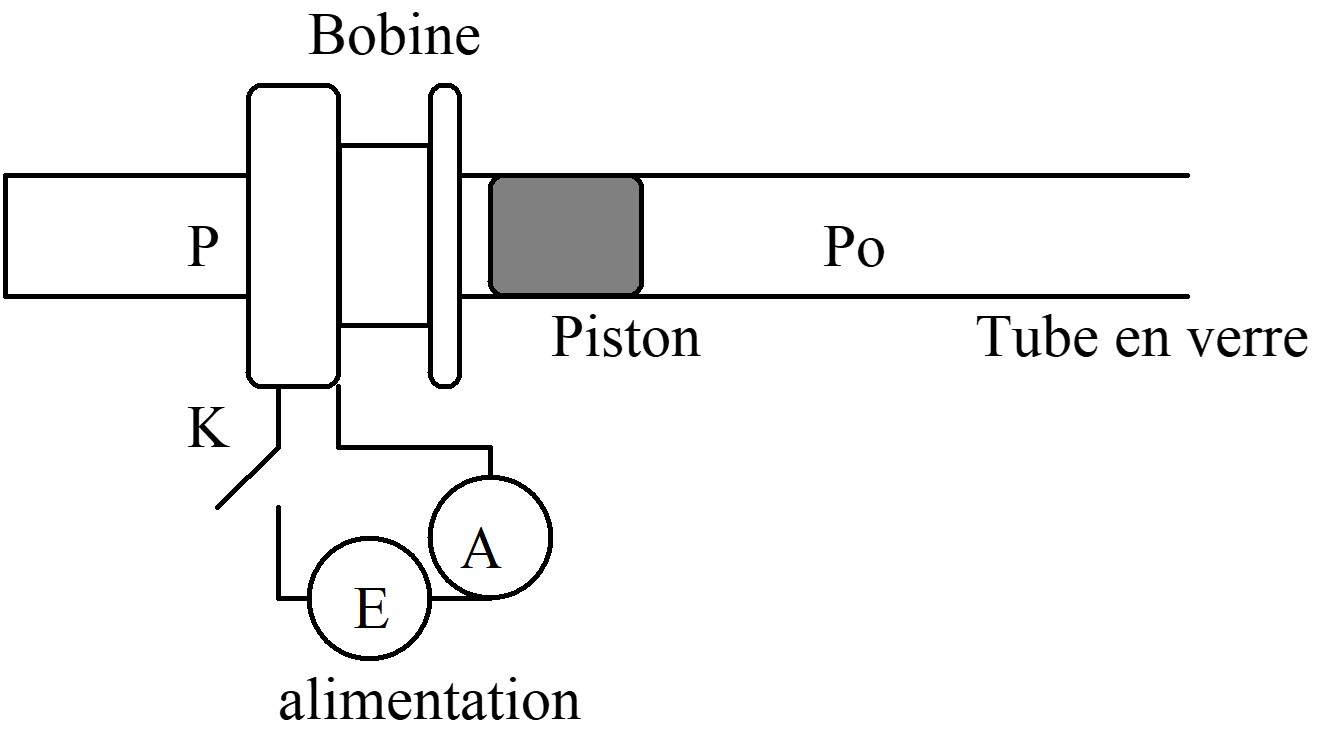
\includegraphics[width=\linewidth]{gamma1}
		\end{center}
	\end{minipage}
	En faisant varier la fréquence du courant dans la bobine, on recherche la
	résonance en amplitude du piston. La fréquence de résonance est liée au
	coefficient adiabatique $\g$ de l'air que l'on se propose de déterminer.

	\subsection{Étude mécanique du piston}
	\noindent
	\begin{minipage}{0.56\linewidth}
		On étudie le système \{piston\} dans le référentiel du laboratoire, supposé
		galiléen. Il est soumis aux forces de pression qui s'exercent sur ses deux
		faces latérales, ainsi qu'à son poids et à la réaction du support, forces
		qui se compensent. Enfin, il est soumis à la force d'excitation magnétique
		$\vv{F}\ind{mag}$ engendrée par la bobine. On suppose cette force
		proportionnelle au courant $i(t)$ circulant dans la bobine selon
	\end{minipage}
	\hfill
	\begin{minipage}{0.40\linewidth}
		\begin{center}
			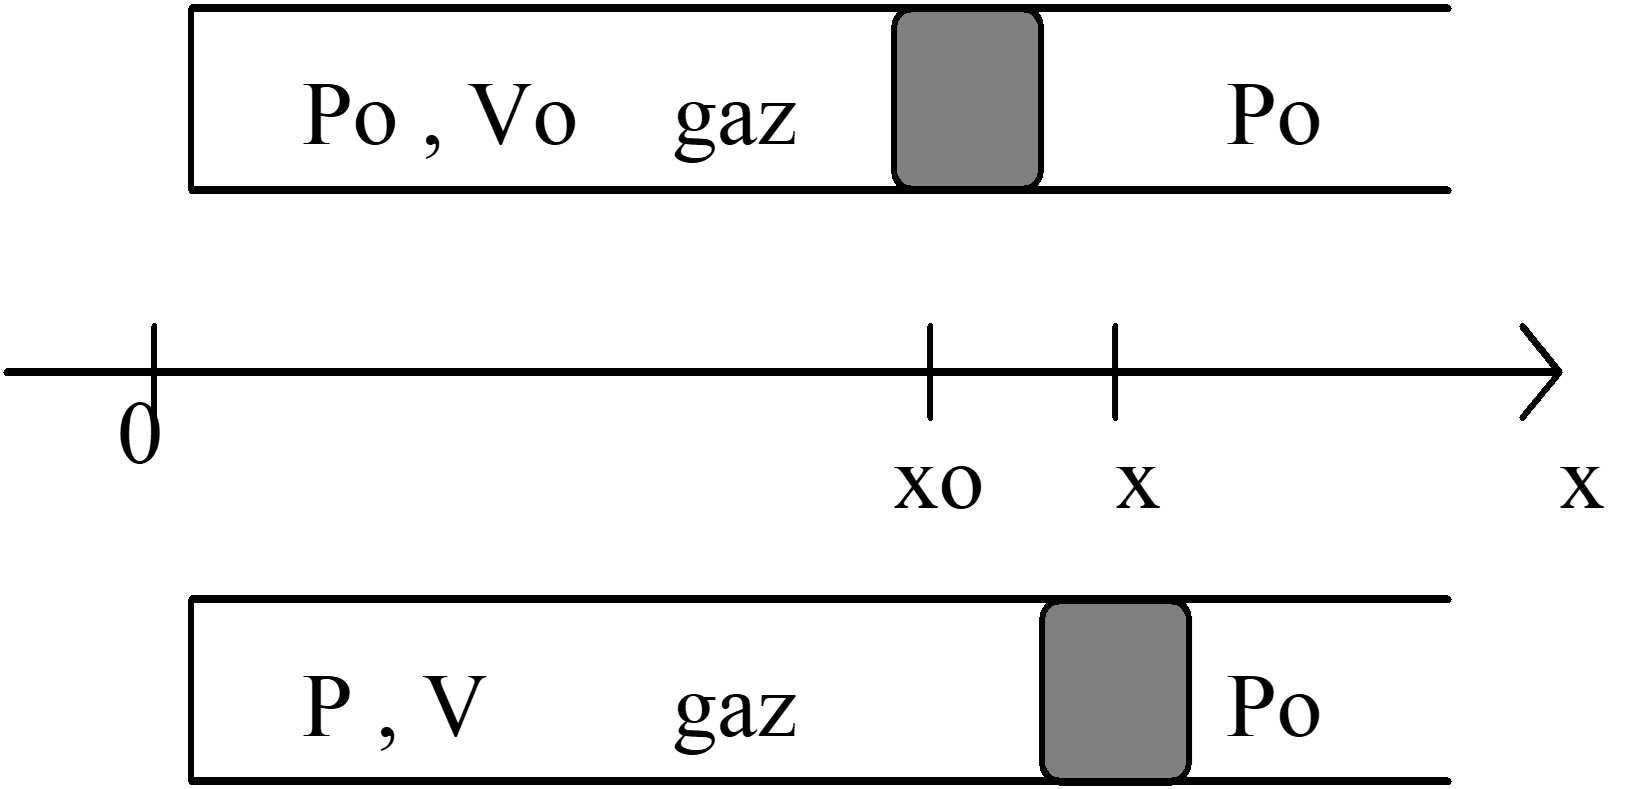
\includegraphics[width=\linewidth]{gamma2}
		\end{center}
	\end{minipage}
	\[
		\Ff\ind{mag} = \beta i(t) \ux
	\]
	avec $\beta$ une constante que l'on ne cherchera pas à déterminer.
	\bigbreak
	Étudions le mouvement du piston selon l'axe horizontal $(Ox)$. À l'équilibre, le
	piston se trouve en $x_0$, la pression étant égale à la pression atmosphérique
	$P_0$ sur chaque face. Le volume fermé de gaz est $V_0$. On considère un petit
	déplacement du piston dans le sens des $x$ croissants. Le volume de gaz fermé
	devient $V$, et la pression qui s'exerce sur la face gauche du piston est $P <
		P_0$ puisque le volume fermé de gaz a subi une détente. En appliquant la
	deuxième loi de Newton en projection selon l'axe $(Ox)$, on obtient~:
	\[
		\boxed{m\xpp = (P-P_0)S + \beta i(t)}
	\]
	où $m$ est la masse du piston et $S$ sa section.

	\subsection{Transformations thermodynamiques subies par le volume fermé de gaz}

	Au cours de l'expérience, les oscillations du piston sont suffisamment rapides
	pour pouvoir supposer que les transformations subies par le gaz sont
	adiabatiques, c'est-à-dire sans échange de chaleur avec l'extérieur. D'autre
	part on assimile le gaz (l'air) à un gaz parfait de coefficient adiabatique $\g$
	constant. Au cours de telles transformations, l'équation d'état du gaz suit la
	loi dite de \textsc{Laplace} telle que
	\[
		PV^\g = C
	\]
	avec $C$ une constante. L'expression différentielle de cette loi est~:
	\[
		\frac{\dd P}{P} + \g \frac{\dd V}{V} = 0
	\]
	On en déduit donc une relation entre la variation de pression $\dd P$ du gaz et
	sa variation $\dd V$ de volume au cours de la transformation.
}

\setcounter{section}{2}
\section{Analyser}
\subsection{Équation différentielle du mouvement}

D'après les caractéristiques du tube, $\dd V=S \dd x$. On suppose toutes les
variations faibles par rapport aux grandeurs de repos, si bien que
\[
	P = P_0 +\dd P \approx P_0 \qqet V = V_0 +\dd V \approx V_0
\]
Sous ces hypothèses, l'expression différentielle de la loi de \textsc{Laplace}
permet d'écrire~:
\[
	\dd P = -\g P_0 \frac{\dd V}{V_0}
\]
Et, en utilisant le fait que $\dd V = S \dd x = S (x-x_0)$,
\[
	\boxed{P-P_0 = \dd P = - \g \frac{P_0}{V_0} \, S \, (x-x_0)}
\]

\setlist[blocQR,1]{leftmargin=10pt, label=\clenumi}
\QR[2]{%
	Donner alors l'équation différentielle du mouvement du piston en $x$
}{%
	On a
	\begin{gather*}
		\left\{
		\begin{array}{rl}
			m \xpp  & = (P - P_0)S + \beta i(t)
			\\
			P - P_0 & = - \gamma \frac{P_0}{V_0}S (x-x_0)
		\end{array}
		\right.
		\quad \Ra \quad
		m \xpp = -\gamma \frac{P_0}{v_0}S^2(x-x_0) + \beta i(t)
		\\\Lra
		\boxed{
			\xpp + \frac{P_0 S^2 \gamma}{m V_0}x =
			\frac{P_0 S^2 \gamma}{m V_0} x_0 + \frac{\beta}{m}i(t)
		}
	\end{gather*}
}

\QR[1]{%
	Déterminer la pulsation propre du mouvement.
}{%
	\begin{gather*}
		\boxed{
			\xpp + \w_0{}^2 x =
			\w_0{}^2  x_0 + \frac{\beta}{m}i(t)
		}
		\quad \Ra \quad
		{\w_0} = \sqrt{\frac{P_0S^2\g}{mV_0}}
	\end{gather*}
}

\QR[2]{%
Montrer que le tracé de la \textbf{fréquence} de résonance au carré en
fonction de $1/V_0$ est une droite de coefficient directeur $a$ dont on
précisera l'expression.
}{%
\[
	\vspace{-15pt}
	\w_0{}^{2} = (2\pi f_0)^{2}
	\Lra
	\boxed{
	f_0{}^{2} = \frac{P_0S^{2}\gamma}{4m\pi^{2}}\frac{1}{V_0}
	}
\]
D'où
\[
	y\tikzmark{yn} = a\tikzmark{an}x\tikzmark{xn} + b\tikzmark{bn}
	\tikz[remember picture, overlay]
	\draw[-stealth, transform canvas={xshift=-6pt, yshift=-6pt}]
	(pic cs:yn) --++ (-10pt,-10pt)
	node[anchor=north east] {$f_0{}^2$}
	;
	\tikz[remember picture, overlay]
	\draw[-stealth, transform canvas={xshift=-10pt, yshift=-6pt}]
	(pic cs:an) --++(-5pt,-10pt)
	node[anchor=north] {$\DS \frac{P_0 S^2 \gamma}{4m\pi^2}$}
	;
	\tikz[remember picture, overlay]
	\draw[-stealth, transform canvas={xshift=0pt, yshift=-6pt}]
	(pic cs:xn) --++(5pt,-10pt)
	node[anchor=north] {$\DS \frac{1}{V_0}$}
	;
	\tikz[remember picture, overlay]
	\draw[-stealth, transform canvas={xshift=3pt, yshift=-6pt}]
	(pic cs:bn) --++(10pt,-10pt)
	node[anchor=north west] {$0$}
	;
\]
\vspace{20pt}
}

\enonce{%
	\subsection{Excitation de l'oscillateur}
	Les frottements étant suffisamment faibles, le facteur de qualité est alors
	grand devant 1, si bien que la pulsation de résonance obtenue
	expérimentalement est très proche de la pulsation propre $\w_0$. On a donc
	accès expérimentalement à la valeur de la fréquence propre du piston.
}

\section{Réaliser}
\subsection{Schéma du montage et alimentation de la bobine}
\begin{tcb}[sidebyside, righthand ratio=.40](expe)<itc>{Montage}
	On alimente la bobine à l'aide d'un GBF sur sa \textbf{sortie amplifiée}
	$\SI{0,5}{\ohm}$), qui peut délivrer environ $\SI{1}{A}$ (nécessaire au
	fonctionnement du dispositif), ce qui est impossible avec la sortie
	classique du GBF.
	\bigbreak
	L'ampèremètre branché en série permet de vérifier l'intensité efficace
	débitée dans le circuit. Il faut qu'elle soit de l'ordre de
	\SIrange{0.8}{0.9}{A}, et toujours inférieure à $\SI{1}{A}$.
	\tcblower
	\begin{center}
		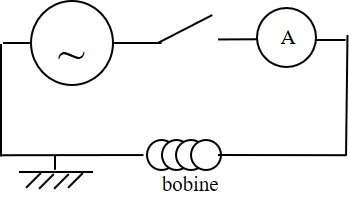
\includegraphics[width=\linewidth]{gamma3}
	\end{center}
\end{tcb}

\begin{tcb}[sidebyside](rapp){Rappel}
	On rappelle que la valeur efficace $S\ind{eff}$ d'un signal $s(t)$ dit
	$T$-périodique est définie par
	\[
		S\ind{eff} = \frac{1}{T} \sqrt{\int_{0}^{T} s^2(t)\dd t}
	\]
	\tcblower
	Pour un signal sinusoïdal comme le courant ici, la valeur efficace est liée
	à l'amplitude $S_0$ selon~:
	\[
		S\ind{eff} = \frac{S_0}{\sqrt{2}}
	\]
\end{tcb}

\subsection{Mode opératoire}
Aller sur \texttt{Capytale}, en cliquant sur
\url{https://capytale2.ac-paris.fr/web/c/4523-1426759}
\begin{tcb}[breakable](expe)<itc>{Mesures}
	\begin{enumerate}
		\item Ouvrir le robinet de la burette, et choisir un volume initial $V_0$
		      grâce à l'aimant. Notez cette valeur de $V_0$ dans la liste
		      \texttt{python} correspondante, et fermer le robinet.
		\item Disposer alors la bobine de manière à ce que son bord se trouve à
		      hauteur du bord du piston.
		\item Allumer le GBF et augmenter le \texttt{level} jusqu'à ce que
		      l'intensité (lue sur l'ampèremètre) soit d'environ
		      \SIrange{0.8}{0.9}{A}.
		\item Chercher la fréquence de résonance, en partant d'une fréquence de
		      $\SIrange{40}{50}{Hz}$ environ et en la diminuant (ne pas descendre
		      sous les $\SI{10}{Hz}$). À la résonance, le cylindre oscille alors
		      avec une relativement grande amplitude.
		\item Noter cette valeur dans la liste \texttt{python} correspondante.
		      Remplir la liste \texttt{Df0} de la plage de valeurs où vous estimez
		      que la résonance se trouve (i.e.\ on a $f_0$ dans $[f_0 -\D, f_0
					      +\D]$)~; l'incertitude-type $u(f_0)$ est alors $\D/\sqrt{3}$.
		\item Ouvrir l'interrupteur pour couper le courant et lire le volume
		      correspondant après oscillation. La différence avec $V_0$ correspond à
		      l'écart à rentrer dans \texttt{DV0}, et l'incertitude-type sera alors
		      \texttt{uV0 = DV0/np.sqrt(3)}.
		\item Déplacer de nouveau le piston en ayant ouvert le robinet, et faire
		      ainsi une série de mesures en faisant varier $V_0$ et en repérant la
		      valeur de $f_0$, sa plage d'existence et la plage d'existence de $V_0$
		      pour chaque valeur de $V_0$.
	\end{enumerate}
\end{tcb}

\section{Valider et conclure}

\setlist[blocQR,1]{leftmargin=10pt, label=\sqenumi}
\QR<[start=1]>{%
	Toujours sur \texttt{Capytale}, remplissez les listes des erreurs
	\textbf{relatives} pour $V_0$ et $f_0$.
}{%
	Voir Capytale~:~\url{https://capytale2.ac-paris.fr/web/c/c758-3021536}.
}

\QR{%
	Créer les variables nécessaires au tracé de ${f_0}^2$ en fonction de
	$1/V_0$.
}{%
	Idem.
}

\QR{%
	Effectuer la régression linéaire avec \texttt{polyfit}, compléter la
	fonction définissant la régression linéaire, et tracer le graphique des
	données relevées avec la régression. Les erreurs à afficher sont les
	incertitudes absolues, pas relatives.
}{%
	Idem.
}

\QR[1]{%
	La régression est-elle valide~?
}{%
	Pour qu'elle soit valide, il faut que les points soient répartis aléatoirement
	autour de la droite, et qu'elle passe par les incertitudes. Sur
	\texttt{Capytale} c'est globalement le cas, par contre la droite ne passe pas
	par 0 même avec les incertitudes. Elle est donc peu fiable.
}

\QR[1]{%
Relever le coefficient directeur $a$ de la droite modélisée. Quelle
est son unité~?
}{%
Pour la valeur, cf.\ Capytale.
\[
	a = V_0{f_0}^2
	\quad \Ra \quad
	[a] = [V_0][f_0{}^2]
	\quad \Lraqud
	\boxed{[a] = \si{cm^3.s^{-2}}}
\]
}

\QR[1]{%
	Déduire, de la partie Analyse, l'expression littérale du coefficient
	adiabatique $\g$ de l'air en fonction du coefficient directeur $a$ de la
	droite modélisée, de la masse $m$ de l'aimant, \textbf{du diamètre $d$
		du piston} et de la pression atmosphérique $P_0$.
}{%
	On isole $\g$~:
	\[
		\gamma = \frac{4\pi^2 m a}{P_0 S^2}
		\Lra
		\boxed{\gamma = \frac{64ma}{P_0 d^4}}
	\]
}

\QR[1]{%
	On a $m = \SI{8,8}{g}$ et $d = \SI{13,97}{mm}$. La pression
	atmosphérique $P_0$ se lit sur le baromètre placé dans la salle (en
	\si{mbar}). Après avoir détaillé les valeurs expérimentales et leurs
	unités correctes sur votre copie, utilisez \texttt{Capytale}, pour
	calculer la valeur expérimentale de $\g$ de l'air. Quelle est son
	unité~?
}{%
	On a, en unités SI,
	\begin{gather*}
		m = \SI{8.8e-3}{kg}
		\quad ; \quad
		P_0 = \SI{982.5e2}{Pa}
		\quad ; \quad
		d = \SI{13.97e-3}{m}
		\quad ; \quad
		a = \SI{8430.51e-6}{m^3.s^{-2}}
		\\\beforetext{D'où}
		\boxed{\gamma = \num{1.27}}
	\end{gather*}
	Avec des calculs ou en analysant la loi de \textsc{Laplace}, on trouve que
	$\gamma$ est \textbf{adimensionné}.
}

\QR{%
	Utiliser le code \texttt{Monte-Carlo} pour estimer la valeur moyenne
	de $a$ et l'incertitude sur la valeur de $a$. En déduire la valeur
	moyenne et l'incertitude sur la valeur de $\g$.
}{%
	Cf.\ Capytale.
}

\QR{%
	Le cours de thermodynamique permettra de déterminer le coefficient
	$\g$ d'un gaz selon qu'il soit un gaz parfait diatomique ou monoatomique. On a
	\[
		\g\ind{dia,théo} = \frac{7}{5}
		\qet
		\g\ind{mono,théo} = \frac{5}{3}
	\]
	Déterminer la bonne valeur théorique par calcul d'écart normalisé. Comparez à
	ce que vous savez des gaz composant l'air (mono- ou diatomique).
}{%
	Idem. On doit trouver le coefficient pour un gaz parfait diatomique, puisque
	l'air est principalement constitué de \ce{N2} et \ce{O2}.
}

\QR[1]{%
	Conclure.
}{%
	Dû à l'usure des tubes et de problèmes d'étanchéité, les mesures sont peu
	précises. On obtient cependant une valeur bien plus proche du gaz diatomique
	que monoatomique.
}

\end{document}
